
\documentclass[12pt]{report}

\usepackage[utf8]{inputenc}
\usepackage[T1]{fontenc}
\usepackage[francais]{babel}
\usepackage{graphicx}
\usepackage{verbatim}

\title{\textbf{Rapport - Projet technologique:\\Hashiwokakero}}
\author{\textbf{Groupe TM2H:}\\Adrien Chinour\\ Camille Meyrignac\\ Louis-Gabriel Barrère}

\begin{document}

\maketitle

\tableofcontents

\chapter{Implantation de la librarie hashi}

\section{Création des fonctions de base}

\subsection{Les fonctions de node.c}
\textnormal{Après avoir compris le principe de base d'une partie hashiwokakero, il a était très facile de définir un \textbf{node}: il est composé de ses coordonnées et de son degré. Les fonctions de node.c sont relativement simples puisqu'elles sont simplement là pour créer, accéder à et supprimer la structure node définie de cette manière:}
\begin{verbatim}
typedef struct node_s {
	int x;
	int y;
	int required_degree;
} *node;
\end{verbatim}

\textnormal{Nous n'avons pas eu de difficulté a réaliser cette partie, surtout que le fichier qui nous était donné comme guide (node.h) contenait toutes les informations pour réaliser les fonctions. Le plus dur dans la création des fonctions de base se trouve dans le game.c}
\subsection{Les fonctions de game.c}
\textnormal{En effet, les fonctions composant game.c ont été un peu plus dur à réaliser. Tout d'abord, il a fallut définir la structure game qui contient les noeuds de la partie, le nombre de noeuds et les ponts.\\ Pour les noeuds, rien de bien compliqué: il suffit de créer un tableau de noeud et de donner à la structure le pointeur sur le premier élément. Pour les ponts, il a fallut un peu plus réfléchir, mais nous avons fini par créer une matrice de la taille du nombre de noeuds par le nombre de directions (c'est-à-dire 4). Voilà à quoi ressemble donc notre structure game:}
\begin{verbatim}
typedef struct game_s {
  int nb_nodes;
  node *nodes;
  int **bridges;
} *game;
\end{verbatim}

\textnormal{Une fois la structure correctement définie, il a fallut réaliser les fonctions de création et de destruction d'une partie. Après quelques tests avec valgrind, tout semblait correct.\\ Nous nous sommes donc attaqués au gros du sujet : les fonctions qui font vivre ces structures game et node (l'ajout de pont, la supression de pont, le test de fin de partie...). Au fur et à mesure de notre avancement, les tests nous ont permis de déceller de nombreux bugs et nous éviter de nombreuses heures de débuggage même si gdb et valgrind nous ont énormément servi durant cette période.\\ Les fonctions les plus complexes qui nous ont demandé beaucoup de temps sont : can\_add\_bridge\_dir et game\_over.}

\subsubsection{La fonction can\_add\_bridge\_dir}
\textnormal{Cette fonction est l'une des plus utiles du jeu : elle permet de savoir s'il est possible ou non d'ajouter un pont. Il faut donc vérifier qu'il y ait un noeud dans la direction et que le pont ne croise pas un autre pont déjà existant. Pour la première vérification c'est assez simple puisque nous disposons déjà d'une fonction qui fait ça. Pour la deuxième vérification, après avoir cherché un bon moment, nous avons choisi de représenter nos ponts sous forme de vecteurs et de vérifier par le calcul vectoriel si notre pont croise un autre pont. \\ Supposons que le vecteur $\overrightarrow{AB}$ est notre pont et le vecteur $\overrightarrow{CD}$ l'autre pont, alors si : $\overrightarrow{AB} \land \overrightarrow{CD} \neq 0$, les deux vecteurs se croisent, mais il faut vérifier s'ils se croisent sur le segment [CD] avec: $\overrightarrow{AB} \land \overrightarrow{AD} \times \overrightarrow{AB} \land \overrightarrow{AC} < 0$\\On a donc une fonction qui prend de la place car il faut récupérer toutes les coordonnées des vecteurs, mais qui est plutôt simple.}

\subsubsection{La fonction game\_over}
\textnormal{Pour la fonction game\_over, il faut vérifier que chaque noeud de la partie à le même degré que son degré requis (assez facile) mais il faut aussi vérifier que l'on peut se déplacer entre nimporte quel noeud grâce au pont. En remarquant que notre partie est un graphe, il suffit de vérifier la connexité de ce graphe. Pour faire cette vérification nous avons utilisé une fonction annexe récursive basé sur 'algoritme de parcours d'un graphe en profondeur}
\begin{verbatim}
static void explore(cgame g, int node_num, bool connected[]){
  connected[node_num] = true;
  for(int i = 0; i < game_nb_dir(g); i++){
    if(get_degree_dir(g, node_num, i) != 0){
      if(connected[get_neighbour_dir(g, node_num, i)] == false)
	explore(g, get_neighbour_dir(g, node_num, i), connected);
    }
  }
}
\end{verbatim}
\textnormal{En gros la fonction parcours un sommet (un noeud), l'ajout à la liste des noeuds visités, puis visite ses voisins non visité. La récursion s'arrète quand le sommet n'a plus de voisin à visiter. Il suffit donc ensuite de vérifier la liste pour savoir si tout les noeuds sont visités}
\section{L'interface terminal}
\textnormal{Lors de l'utilisation des game.o et node.o (puisque game.c et node.c n'étaient pas encore codés), nous avons dû utiliser quelque chose de suffisament visuel pour pouvoir détecter les éventuelles erreurs : une interface texte. Il a donc fallut créer une fonction qui prennait en paramètre la taille du jeu (size), un tableau double (grille[size][size]) où chaque case du jeu correspond à une valeur et le jeu lui même (jeu) définit par la structure game.
Voici l'affichage principal de la grille je jeu :}
\begin{verbatim}
for(int y = size-1; y >= 0; y--){
  for(int x = 0; x < size; x++){
    switch (grille[x][y]){
      case -1: printf(" .  "); break;
      case -2: printf(" +  "); break;
      case -3: printf(" #  "); break;
      default: printf(" %d  ", grille[x][y]); break;
    }
  }
}
\end{verbatim}
On peut voir que grille[x][y] peut avoir pour valeur :
\begin{itemize}
\item -1 : cas où l'on affiche un espace sans pont (.)
\item -2 : cas où l'on affiche un pont simple (+)
\item -3 : cas où l'on affiche un pont double (\#)
\item ? : toute autre valeur correspond au degré d'un noeud, on l'affiche
\end{itemize}
Nous avons donc regardé la partie et corrigé les problèmes avec ces lignes, l'affichage permettant alors de connaître toute la composition du jeu.

\chapter{Caprice des profs}
L'utilisation de 4 directions et 2 ponts maximum n'étant pas suffisante, on a dû implémenter les 8 directions du jeu et 3 ponts posables (il est facile de mettre autant de ponts que souhaité à présent).
On a ajouté à la plupart des fonctions les variables nb\_max\_bridges (nombre maximum de ponts posables) et nb\_dir (nombre de directions) dans une structure pour permettre de détecter le type de partie que l'on souhaite.Voici la structure concernée:
\begin{verbatim}
typedef struct game_s {
  int nb_nodes;
  node *nodes;
  int **bridges;
  int nb_dir;
  int nb_max_bridges;
} *game;
\end{verbatim}
Il a fallut dans ce cas se servir de l'outil git diff pour savoir où il fallait changer quelque chose. Les changements ont été fait dans des switch pour ajouter les directions NW; SW; SE; NE et traiter ces cas. Ainsi, la fonction d'affichage a dû être enlevée puisqu'elle ne traitait pas ces ajouts, donc elle a été refaite entièrement pour pouvoir traiter chaque cas, le précédent affichage étant trop sale. Cependant, l'implémentation des directions et des nouveaux ponts s'est fait assez rapidement, car les autres fonctions étaient déjà faites. Globalement, la plus grosse difficulté était de repérer où faire les changements.


\chapter{Solveur}
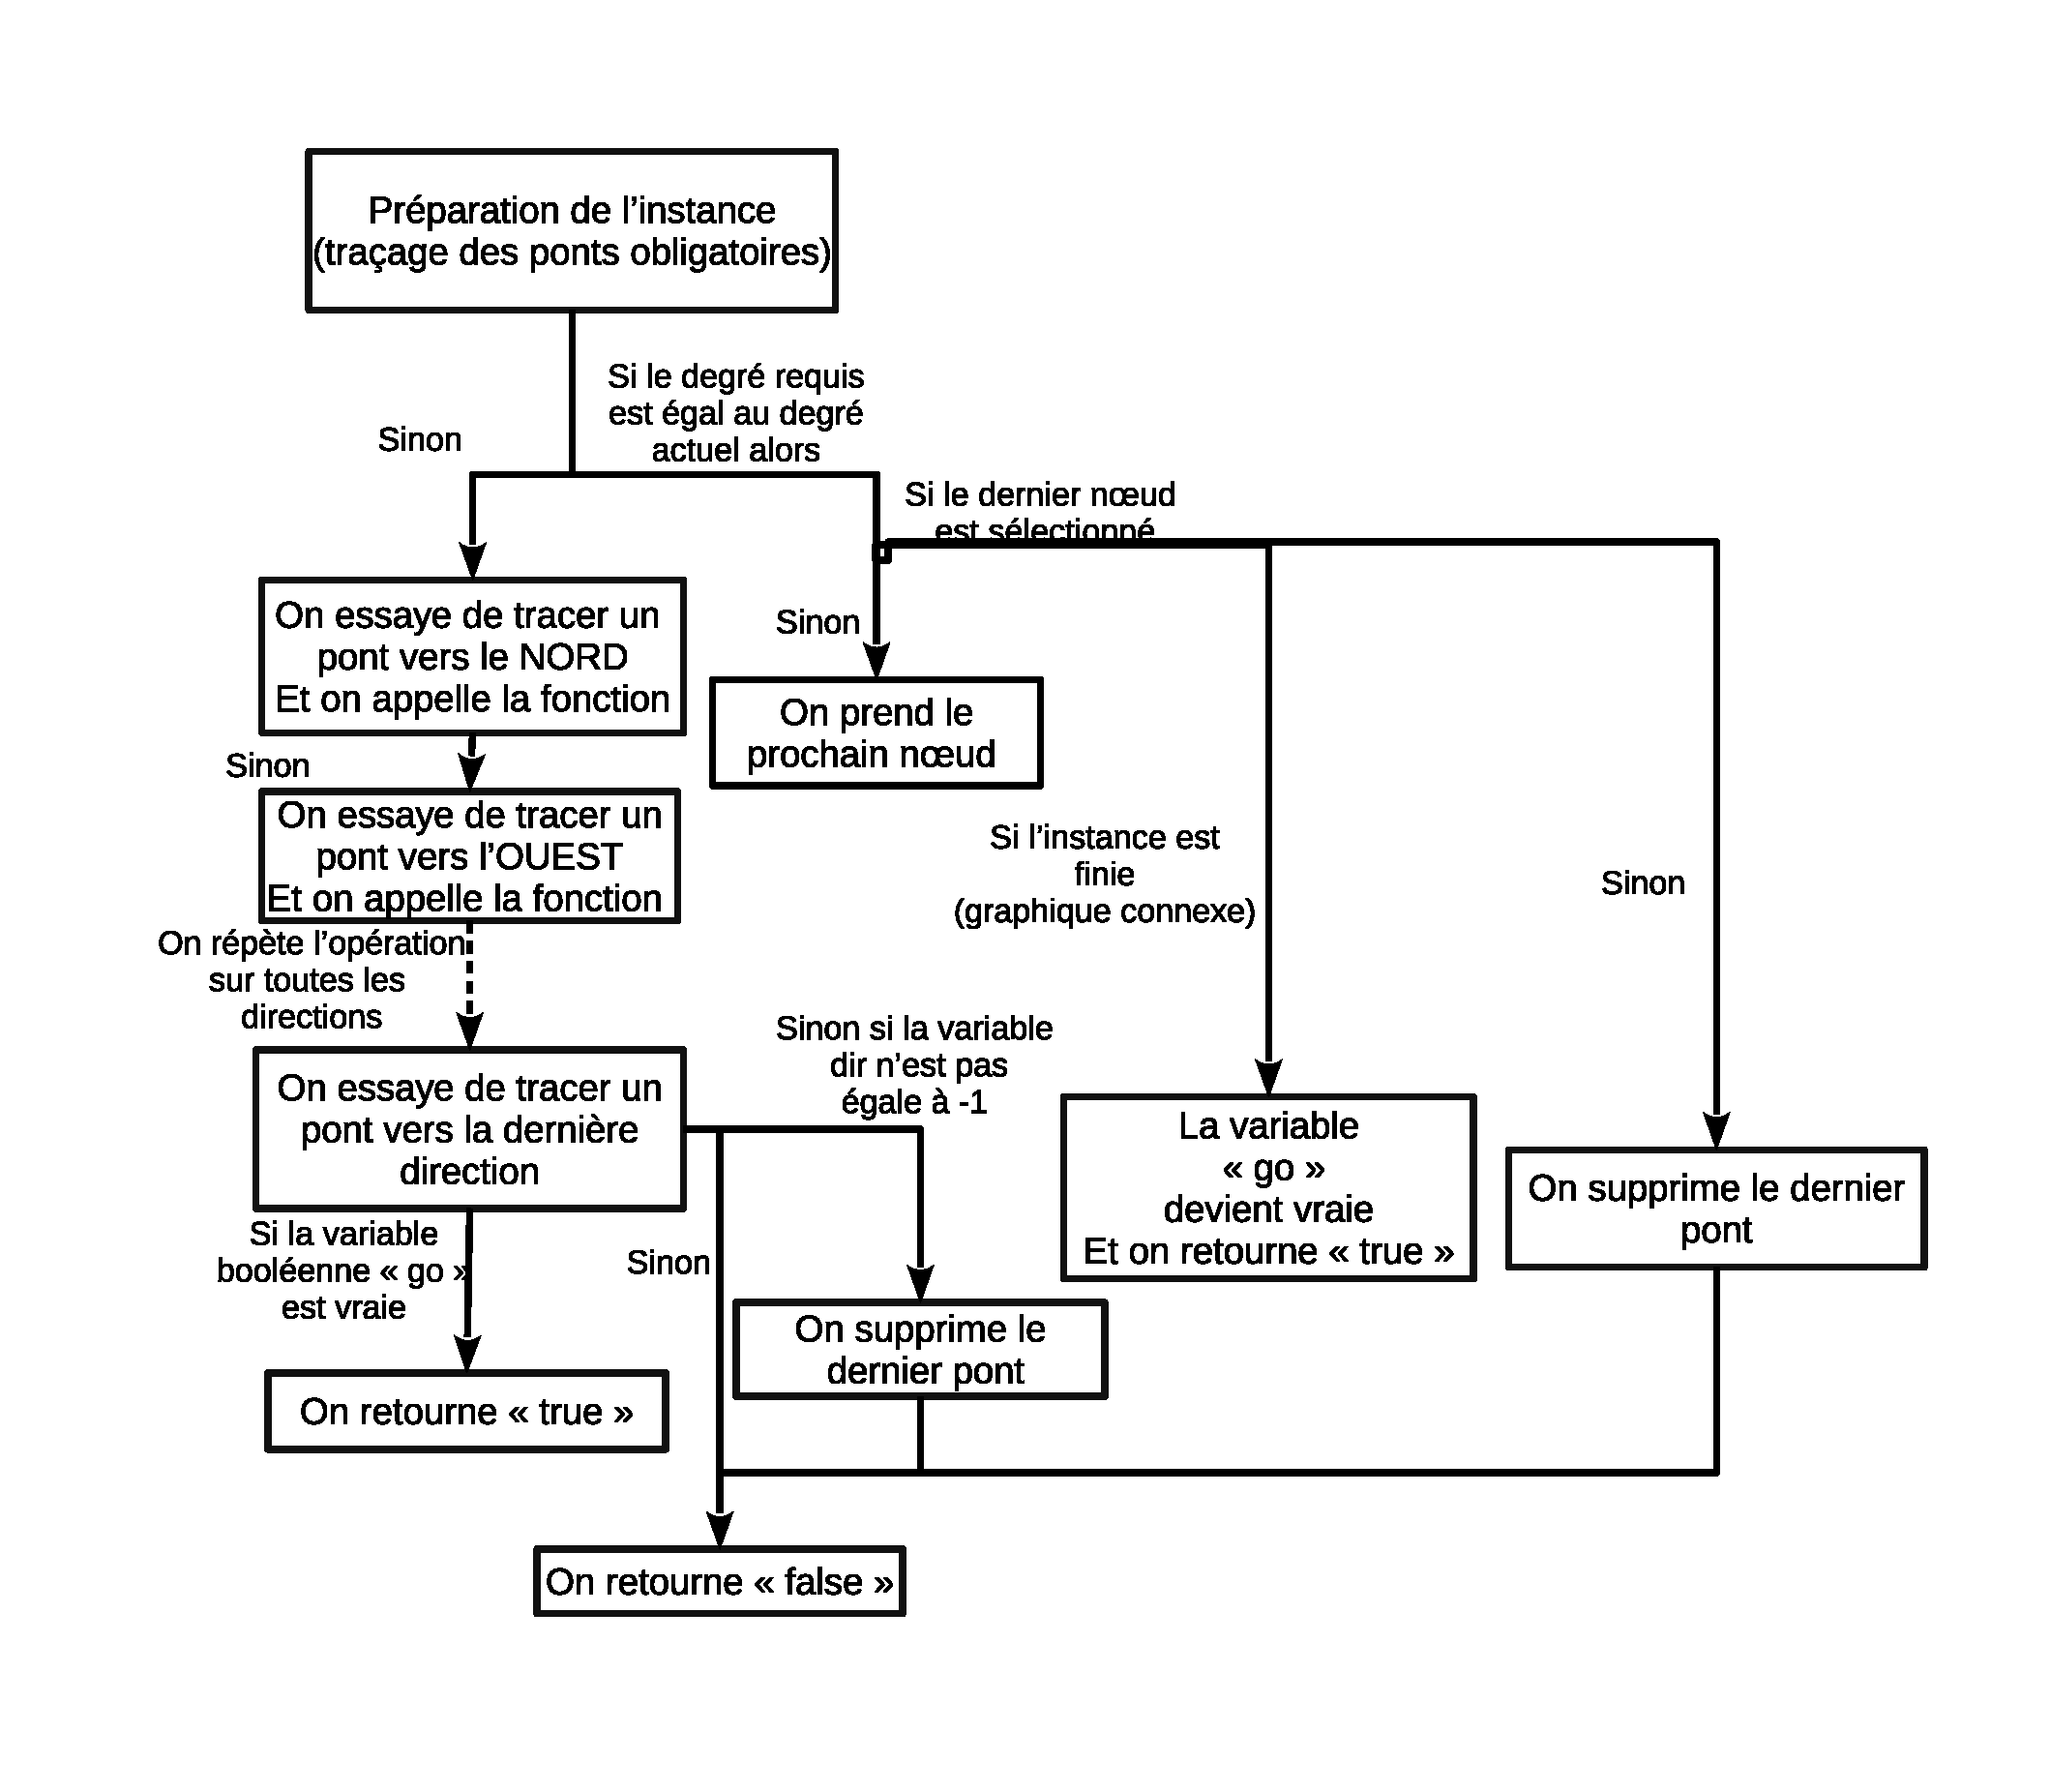
\includegraphics[width = 1.00\textwidth]{explication_solveur.eps}
\section{Explication du graphique}

La préparation de l'instance consiste à tracer les ``ponts obligatoires'',cela concerne les îles qui n'ont qu'une possibilité de liens,
on a déterminé plusieurs cas:
\begin{itemize}
\item Deux îles ne peuvent pas se completer totalement mutuellement, celà formerait un bloc connexe.
\item Si une île a un nombre de ponts possible maximum (en fonction des voisins possiblement atteignable) égale à son degré requis on doit tracer tout ses ponts.
\end{itemize}

Les arguments de la fonction sont:
\begin{itemize}
\item l'instance de jeu (g)
\item le numéro de l'île où nous allons appliquer nos opérations (node\_num)
\item la direction du dernier pont posé utile quand on dépile pour retirer le dernier pont (dir)
\item une variable indiquant si la solution a été trouvée (go)
\end{itemize}

\section{Possibilité d'amélioration}
Pour améliorer ce solveur on pourrait refaire le processus de ``ponts obligatoire'' à chaque fois que l'on fait une action mais celà implique d'avoir une sauvegarde de l'état du jeu pour que lorsque l'on dépile on puisse retirer les ponts posés par ce processus. On a aussi essayé de rajouter une vérification de la possibilité de connexité à chaque fois que l'on pose un pont,comme ça il ne pourrait pas se former de blocs isolés.

\chapter{Interface graphique}
\section{Structure principale de la partie graphique}
La partie graphique est composé de 4 fonctions principale ayant des utilités différentes:
\begin{itemize}
\item Une fonction d'initialisation de l'environnement graphique, qui gère la création des textures, le chargement d'une instance de jeu etc
\item Une fonction de rendu qui s'occupe d'afficher les textures
\item Une fonction qui s'occupe des évenements
\item Une fonction de désallocation qui s'occupe de désallouer les textures et l'instance de jeu
\end{itemize}

\section{Capacités de l'application}
On a réussi à avoir un jeu qui marche avec 4 ou 8 directions et de 2 à 4 ponts, avec d'autres fonctionnalités comme un affichage des ponts possible en passant le pointeur de la souris dessus, des boutons permettant de remettre la partie à 0, de tricher avec le solveur, de charger une partie générée aléatoirement et de sauvegarder. Et si on augmente le nombre de ponts maximum il ne faut rien modifier dans l'affichage.

\section{Problèmes de développement}
La SDL comportant diverses fuites mémoire il a été très dur de déterminer d'où venaient les fuites mémoires avec Valgrind nous avons dû faire des efforts supplémentaires pour lire le code. Ce moment était celui où l'on avait le plus besoin de tous écrire dans le même fichier mais ce problème a été aisément réglé avec l'aide de GIT et sa fonctionnalités de fusion de fichiers, ça a été le moment où l'on a le plus eu besoin de cette fonctionnalités comme le montre le log de GIT.

\section{Affichage du jeu}
Notre projet ressemble à ça:\\

\includegraphics[width = 1.00\textwidth]{capture.eps}



\chapter{Portabilité sur Android}
\section{Introduction}
\textnormal{La première partie du travail a était d'ajouter le répertoire android à notre projet. Ensuite nous avons modifié le fichier qui permet de compiler notre programme pour android (android.mk). Puis modifié la variable YOUR\_SRC\_FILES qui correspond à nos fichier C utile à l'application android. Plutôt que de dupliquer ces fichiers nous avons simplement donner le chemin des fichiers utiliser pour la compilation standard.\\Ensuite il a fallut modifier et ajouter du code a nos fichiers comme par exemple pour la gestion des évènement sous SDL ou la lecture de fichier afin que la compilation se déroule sans erreur.}
\section{Gestion des évènements SDL}
\textnormal{Pour la gestion des évènements il a falut ajouter un \#ifdef pour séparer les évènement liés à un ordinateur et ceux qui sont liés à android, avec SDL il est très facile de faire ça gràce au évènement prédéfini pour android:}
\begin{verbatim}
#ifdef __ANDROID__
  if (e->type == SDL_FINGERDOWN) {
    /* action liée à une pression du doigt */
  }
#else
  if(e->type == SDL_MOUSEBUTTONDOWN){
    /* action liée à un clic de souris */
  }
#endif
\end{verbatim}
\section{Lecture de fichier sur android}
\textnormal{Après avoir compilé une première fois notre programme et testé ça sur un smartphone android l'application s'ouvrait et se fermait directement.\\Ce problème est dû au fait que les fonctions de lecture de fichier en particulier fopen ne fonctionne pas sur android, nous avons donc utilisé les fonctions de SDL qui corrige l'ouverture de fichier et nous a permis d'avoir une première version qui fonctionne sur android. Mais la fonction de sauvegarde qui fonctionnait avant sur ordinateur ne marche plus correctement pour les ponts et ne fonctionne pas sur android non plus.}

\end{document}
